\paragraphn{Preactivations analysis 1 - Distributions}
We concluded the quantitative analysis leaving an open question: does the pre-KENN network adapt its predictions to KENN's action? To answer this question, we can start by examining the distribution of the preactivations of every final model. Each distribution will be split into two graphs to simplify the comparison by separating positive and negative predictions using different scales. Figure~\ref{fig:baseline_distrib} shows the distributions of the baseline model that will be used as a reference point. The values of $x$ are the preactivations of each type of each example, while the $y$ represents the frequency of a bin of preactivations.

We will start by comparing the positive predictions. In Figure~\ref{fig:kenn_pos_distrib} we can find the positive distributions of the KENN-based models. The first thing we can observe is that each KB mode produces very different pre-KENN distributions. If we look at the means (Bottom Up: 2.706, Top Down: 3.633, Hybrid: 2.227) and standard deviations (Bottom Up: 1.737, Top Down: 2.190, Hybrid: 1.434), we can also assert that they differ a lot from the baseline positive distribution (mean: 4.246, standard deviation: 2.228). On the contrary, the situation is completely different when looking at the post-KENN preactivations, since the intervention of KENN makes the distributions more similar to each other (means: 4.100$\pm$0.043, standard deviations: 2.058$\pm$0.038) and to the baseline. The same phenomenon can be observed by comparing the negative distribution of the baseline in Figure~\ref{fig:baseline_neg_distrib} to the pre-KENN and post-KENN negative distributions in Figure~\ref{fig:kenn_neg_distrib}.

\begin{figure}[H]
     \centering
     \begin{subfigure}{0.5\textwidth}
         \centering
         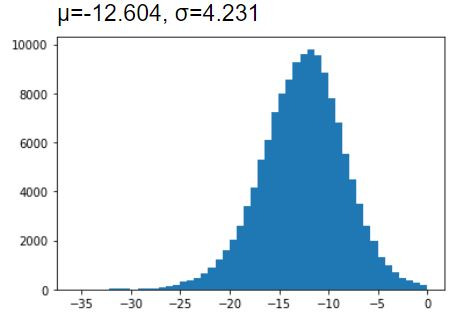
\includegraphics[width=\textwidth]{figures/baseline_neg.JPG}
         \caption{Negative preactivations}
         \label{fig:baseline_neg_distrib}
     \end{subfigure}
     \hfill
     \begin{subfigure}{0.475\textwidth}
         \centering
         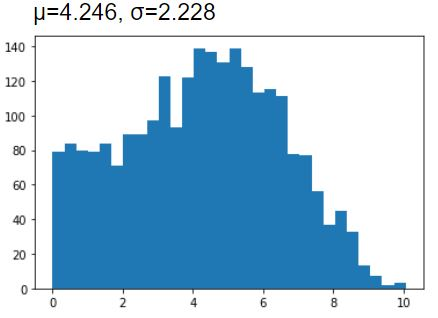
\includegraphics[width=\textwidth]{figures/baseline_pos.JPG}
         \caption{Positive preactivations}
         \label{fig:baseline_pos_distrib}
     \end{subfigure}
        \caption{Distribution of the baseline preactivations computed on the dev set of FIGER}
        \label{fig:baseline_distrib}
\end{figure}


\begin{figure}[H]
    \centering
    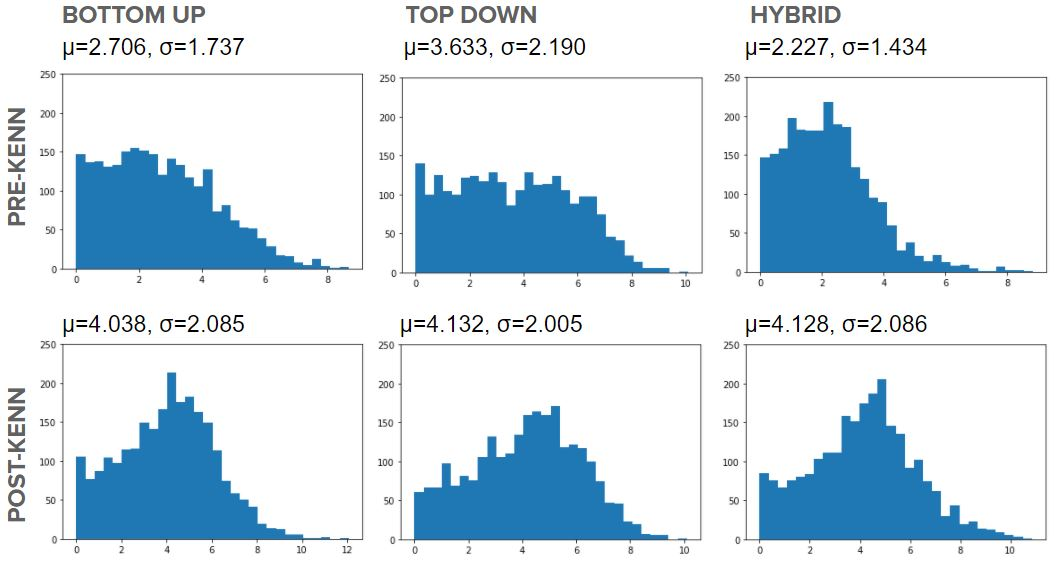
\includegraphics[scale=.53]{figures/kenn_pos_distrib.JPG}
    \caption{Distribution of the pre-KENN and post-KENN positive preactivations for each KB mode. Computed on the dev set of FIGER.}
    \label{fig:kenn_pos_distrib}
\end{figure}

\begin{figure}[H]
    \centering
    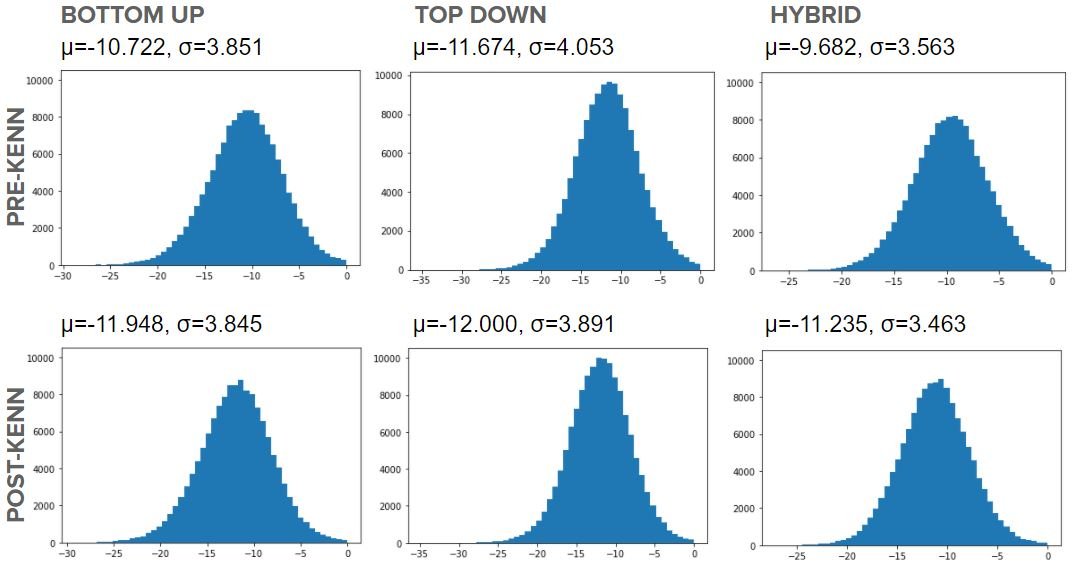
\includegraphics[scale=.53]{figures/kenn_neg_distrib.JPG}
    \caption{Distribution of the pre-KENN and post-KENN negative preactivations for each KB mode. Computed on the dev set of FIGER.}
    \label{fig:kenn_neg_distrib}
\end{figure}

\paragraphn{Preactivations analysis 2 and 3 - FSM and Sankey diagrams}
The analysis of the Finite State Machines and the Sankey diagrams can help to understand how the pre-KENN and post-KENN preactivations are modified depending on types F and S involved in the same clause, thus providing other insights into the suspicion of adaptation emerged in the previous study.

Starting from the Bottom Up mode, we can find the FSM and the Sankey diagram in Figure~\ref{fig:transitions_bottom_up}. We remind that a Bottom Up clause will always produce a positive delta on F and a negative delta on S. Indeed, F1S0 is a sink vertex of the Bottom Up FSM because F can never be decreased and S can never be increased in a Bottom Up setup. By analyzing the information of the transitions, we can observe that:
\begin{enumerate}
    \item The percentages of wrong transitions represent a minority.
    \item The probability of remaining in the forbidden state (i.e., F0S1) is 0.03. This is reasonable because the forbidden state represents also a clause violation (i.e., 1$\to$0) for this KB mode, so KENN will always try to modify the predictions to reach another post-KENN state. In these cases, the percentages of correctness show that the outgoing transitions from F0S1 never lead to worse predictions, but this is trivial since it is a wrong state by definition.
    \item The statistics about the transition F0S1$\to$F1S0 are quite counterintuitive since F and S are reversed correctly in 43.1\% of cases. The fact that the pre-KENN network predicts F as negative and S as positive when the target is the opposite is curious. It is plausible that the pre-KENN network learned that a type F usually receives one or more positive boosts, so it produces an initial negative prediction being aware that KENN will correct the final value. 
    \item The transition F0S0$\to$F1S0 could seem weird too. It has a probability of 0.01 and a percentage of correctness of 84.3\%. Some of these transitions are due to the fact that in the Bottom Up mode a type F is involved in multiple clauses, so the positive boost could derive from one or more siblings of S. However, after an investigation, it emerged that there are several examples of transitions F0S$_{1,...,n}$0$\to$F1S$_{1,...,n}$0 where F becomes positive thanks to the aggregated boost of its negative children. In particular, on a total of 500 F0S0$\to$F1S0 transitions, in 78 of them the effect of a single S was sufficient to enhance F. Even this behavior could be explained by the fact that the pre-KENN network learned that F is used to receive positive boosts.
\end{enumerate}


\begin{figure}
     \centering
     \begin{subfigure}{0.7\textwidth}
         \centering
         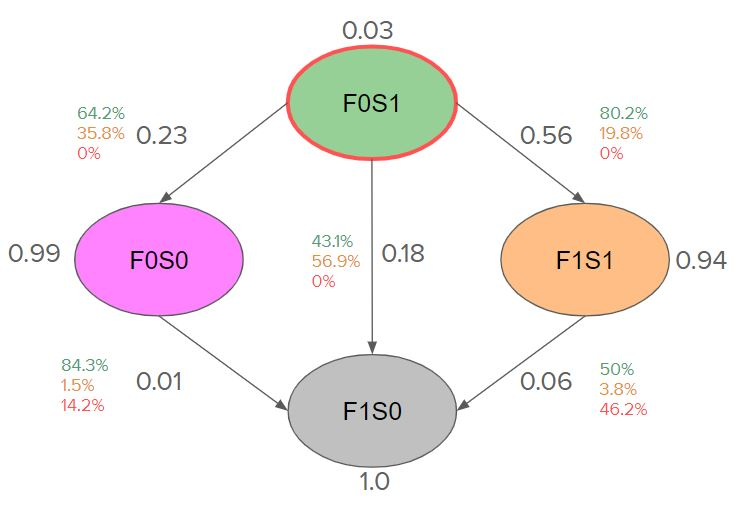
\includegraphics[width=\textwidth]{figures/fsm_bottom_up.JPG}
         \caption{FSM}
         \label{fig:fsm_bottom_up}
         \vspace{15px}
     \end{subfigure}
     \vfill
     \begin{subfigure}{0.6\textwidth}
         \centering
         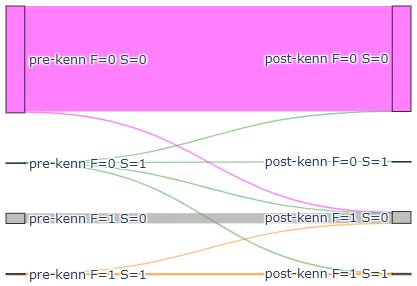
\includegraphics[width=\textwidth]{figures/sankey_bottom_up.JPG}
         \caption{Sankey diagram}
         \label{fig:sankey_bottom_up}
     \end{subfigure}
        \caption{FSM and Sankey diagram of the Bottom Up mode on the dev set of FIGER.}
        \label{fig:transitions_bottom_up}
\end{figure}

The FSM and the Sankey diagram of the Top Down mode are shown in Figure~\ref{fig:transitions_top_down}. The first thing we can notice is that the transitions of the FSM have opposite directions with respect to Bottom Up, so the sink vertex becomes F0S1. Looking at the statistics of the transitions, we can observe that:
\begin{enumerate}
    \item The percentages of wrong transitions represent a minority.
    \item The incoming transitions of the forbidden state have null probabilities when starting from F0S0 or F1S1, and near-zero probability when the pre-KENN state is F1S0. This is a very interesting fact, since it means that the pre-KENN network produces predictions such that KENN cannot generate a boost that leads to the forbidden state.
    \item Even if in this KB mode the pre-KENN state F1S0 may represent a clause violation (i.e., 1$\to 0 \vee ... \vee 0$) that KENN will try to correct, we can still find some examples of self-loop transition. Note that the high probability of 0.867 is due to the fact that in a Top Down clause the consequent is a disjunction of siblings. However, if we exclude from the count the cases in which a sibling of S is positive, we still have a high probability of 0.512 of self-loop. This means that the pre-KENN network learned to generate preactivations that prevent the effect of KENN when the desired output is F1S0.
    \item If we look at the Sankey diagram in Figure~\ref{fig:sankey_top_down}, we can see that the pre-KENN state F0S1 (i.e., the sink node) is missing. In this case too, the reason can be found in the fact that the pre-KENN network is aware that KENN will not be able to change the final predictions.
\end{enumerate}

\begin{figure}
     \centering
     \begin{subfigure}{0.7\textwidth}
         \centering
         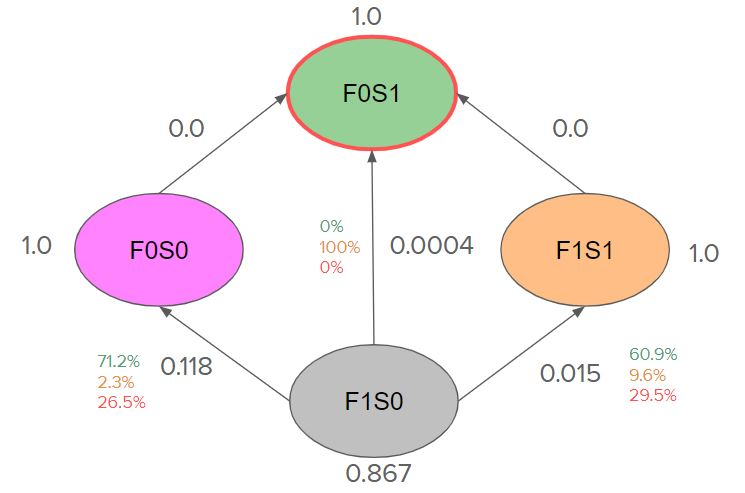
\includegraphics[width=\textwidth]{figures/fsm_top_down.JPG}
         \caption{FSM}
         \label{fig:fsm_top_down}
         \vspace{15px}
     \end{subfigure}
     \vfill
     \begin{subfigure}{0.6\textwidth}
         \centering
         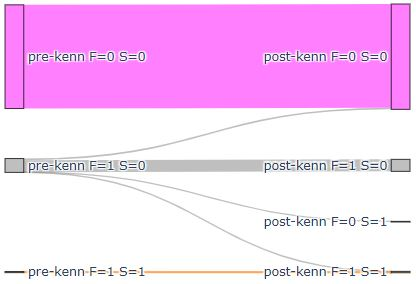
\includegraphics[width=\textwidth]{figures/sankey_top_down.JPG}
         \caption{Sankey diagram}
         \label{fig:sankey_top_down}
     \end{subfigure}
        \caption{FSM and Sankey diagram of the Top Down mode on the dev set of FIGER.}
        \label{fig:transitions_top_down}
\end{figure}

Finally, we can find the transitions of the Hybrid mode in Figure~\ref{fig:transitions_hybrid}. The FSM transitions are bidirectional because they are inherited from Top Down and Bottom Up. The consequence is that there are no sink nodes and all the transitions become potentially available. The considerations we can make by observing the figures are that:
\begin{enumerate}
    \item The percentages of wrong transitions represent a minority.
    \item Similarly to what happens in the Top Down, the probability to make a transition into the forbidden state is null.
    \item The probability of remaining in the forbidden state is very low like in the Bottom Up.
    \item The Sankey diagram is denser than those of Bottom Up and Top Down, since it is constituted by the mix of their transitions.
\end{enumerate}

\begin{figure}
     \centering
     \begin{subfigure}{0.7\textwidth}
         \centering
         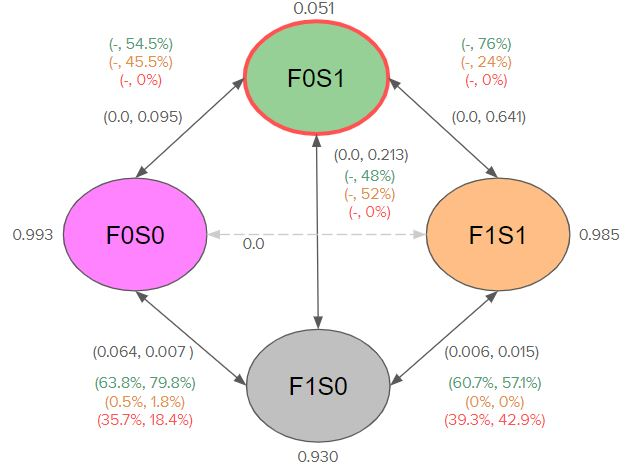
\includegraphics[width=\textwidth]{figures/fsm_hybrid.JPG}
         \caption{FSM - perecentages and probabilities are reported as \textit{(x, y)}, where \textit{x~=~value~of~down-to-up~transition} and \textit{y~=~value~of~up-to-down~transition}  }
         \label{fig:fsm_hybrid}
         \vspace{15px}
     \end{subfigure}
     \vfill
     \begin{subfigure}{0.6\textwidth}
         \centering
         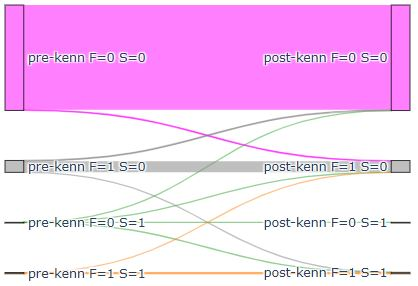
\includegraphics[width=\textwidth]{figures/sankey_hybrid.JPG}
         \caption{Sankey diagram}
         \label{fig:sankey_hybrid}
     \end{subfigure}
        \caption{FSM and Sankey diagram of the Hybrid mode on the dev set of FIGER.}
        \label{fig:transitions_hybrid}
\end{figure}

A final consideration can be done by comparing the three Sankey diagrams: even if their starting states are quite different, their final states become very similar. This fact is analogous to what we observed when comparing the pre-KENN and post-KENN preactivations.

\paragraphn{Preactivation analysis - Conclusion}
This study brought to light several aspects that confirmed the suspicion of adaptation. In the first analysis we saw that while the pre-KENN distributions had relevant differences, the post-KENN distributions became more similar to each other and to the baseline. We then detected other evident signals of adaptation by analyzing the transitions of the FSMs and the Sankey diagrams. Considering the Bottom Up mode, the most representative examples can be found in the transitions F0S1$\to$F1S0 and F0S0$\to$F1S0, where the pre-KENN network seems to be aware of the boost that will be produced on F by KENN. Even more interesting is the situation of the Top Down. Here, the strongest adaptation signals are given by the absence of F0S1 (i.e., sink node) as pre-KENN state in the Sankey diagram and by the high probability of not correcting a violated clause (i.e., self-loop on F1S0).